
In a first step, we evaluated the covariance of the cryptocurrencies (BTC, ETH, XRP, LTC and the CMC200 index) and the 10 year treasury bond (TNX). The results are depicted in Figure \ref{fig:cov} below. We found small ($\leq$0.0021, ignoring covariance with oneself), positive values throughout. The magnitude  is not significant to interpret. Instead, we focus on the sign. All values are positive, indicating a positive relation of prices. Of most interest are the covariances of the 10 year tresury bond with the cryptocurrencies. These values are allocated along the along the bottom and right edge in light pink, indicating very small values, close to zero. The covariance of two variables are close to zero if either both values are very small or if there is no relationship. Refering back to Figure \ref{fig:mean} we see that indeed the mean values of are variables are small ($<$0.003). We can therefore conclude that the risk free rate and cryptocurrencies are probably moving in the same direction.

\begin{figure}
    \centering
    \textbf{\caption{Covariance}}
    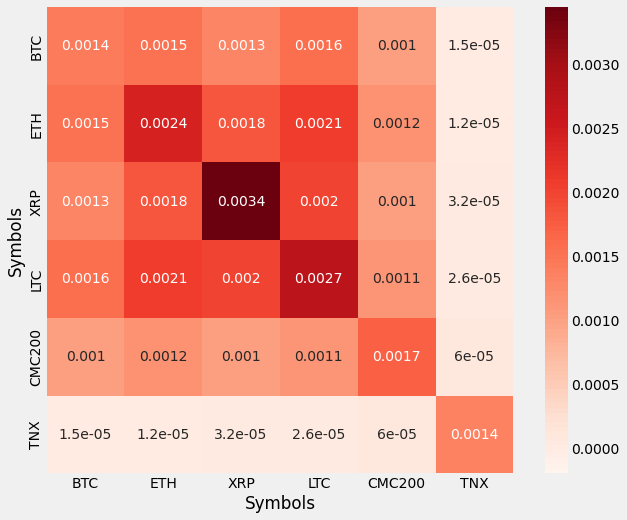
\includegraphics[width=\textwidth,height=\textheight,keepaspectratio]{images/covariance_heatmap.png}
    \label{fig:cov}
    \note{\textit{Note.} Own representation.}
\end{figure}


The correlation between the 10yr treasury yield and other cryptocurrencies is very weak and shows negligible correlation.
The interesting fact is if we compare BTC to other cryptos we see very high positive correlation.


As seen from the results the correlation between the 10yr treasury yield and other cryptocurrencies is very weak
For them to be at least moderatily correlated, the Spearman correlation coefficient would have to be greater than 0.40 in absolute terms.
We conclude that there is no significant correlation between interest rate hikes and cryptocurrency exchange rates